\chapter{NOTICIAS PODCAST}

\section{\textquestiondown Que es feed de noticia?}

El feed \footnote{feed: Suministrar informaci\'{o}n} puede ser m\'{a}s que t\'{i}tulos
y enlaces, esto permite a los usuarios obtengan las \'{u}ltimas actualizaciones del sitio
a diferentes dispositivos enviados desde un sitio web.

Los feeds pueden ser cualquier cosa de pocos titulares y enlaces a historia a todo
el contenido del sitio, despojados de su trazado y con metadatos aplicados generosamente.
Sindicaci\'{o}n de contenidos permite a los usuarios experimentar un sitio en varios 
dispositivos y ser\'{a}n notificados de cambios a trav\'{e}s de una variable de servicios. 
Puede variar desde una simple lista de enlaces enviados desde un sitio a otro a los 
inicios de la Web Sem\'{a}ntica.\cite{hammersley2005developing}

RSS y Atom son XML formatos para mensajes y otra informaci\'{o}n que es actualizada 
frecuentemente. Los documentos que son escritos en estos formatos son llamados newfeeds
or feed.\cite{wittenbrink2005rss}

Se define RSS \footnote{RSS: Really Simple Syndication} como un formato basado en XML 
\footnote{XML:Extensible Markup Language: designado para almacenar y transportar datos} 
para compartir contenido del sitio web.

Si un sitio web quiere compartir y publicar parte de su contenido a otros sitios en el
mismo tiempo, el editor puede crear un documento RSS. Este documento se puede publicar
en el sitio web y cualquier usuario puede leer y utlizar diferentes sitios al mismo 
tiempo. \cite{zeki2004rss}

Se utiliza la tecnolog\'{i}a feed de noticias para tener al usuario a los \'{u}ltimos
contenidos en la aplicaci\'{o}n web y este pueda notificarle via correo electr\'{o}nico
del mismo con el t\'{i}tulo, descripci\'{o}n y categor\'{i}a al que pertenece.

\section{Sintaxis: RSS como XML formato}

Para muchos desarrolladores \textquotedblleft XML\textquotedblright y \textquotedblleft
RSS\textquotedblright son sin\'{o}minos. Se utiliza ambas tecnolog\'{i}as para el 
intercambios de informaci\'{o}n en la Web.

Muchos sitios web identifican sus fuentes de noticias a trav\'{e}s de un bot\'{o}n
de color naranja marcado \textquotedblleft XML\textquotedblright. Para muchos usuarios,
y tambi\'{e}n para muchos desarrolladores \textquotedblleft XML\textquotedblright  y
\textquotedblleft RSS\textquotedblright son sin\'{o}nimos. De hecho, todas las versiones
del formato RSS y Atom son XML aplicaciones. Desde XML en s\'{i} es un metalenguage para
definir idiomas par el intercambio de informaci\'{o}n en la Web, los formatos de fuentes
son tambi\'{e}n a menudo se llama \textquotedblleft dialectos XML\textquotedblright  o 
\textquotedblleft XML vocabularios \textquotedblright. A la fecha, RSS es el vocabulario, 
excepto XML de mayor \'{e}xito para tal XHTML, la versi\'{o}n XML de HTML.\cite{wittenbrink2005rss}

Se identifica un icono de color naranja que contiene en su interior un circulo y dos
lineas curvas de color blanco para conocer que la aplcaci\'{o}n web cuenta con 
subscripci\'{o}n.

\section{RSS 0.90}

Con RSS es posible integrar t\'{i}tulos desde otros sitios en la portada. Los 
usuarios deberian personalizar y suscribirse a un n\'{u}mero de canales que 
ofrece un canal de noticias RSS.


RSS fue inicialmente una abreviatura de \textquotedblleft RDF Site Summary\textquotedblright.
Con RSS, es posible integrar los titulares de otros sitios con enlaces a estos sitios en el 
portal. El usuario puede personalizar el portal y suscribirse a un n\'{u}mero de sitios que
ofrecen datos RSS. De esta manera, My Netscape ten\'{i}a a su disposici\'{o}n una gran 
cantidad de contenidos adicional, que mantiene a los usuarios en el sitio ya; los proveedores
de datos RSS recibida tr\'{a}fico en el objetivo adicional m\'{a}s importante de muchos
sitios web en los tiempos de la boom de las punto-com. Puesta que es f\'{a}cil de convertir
RSS a HTML. Otros sitios pronto empezaron a utilizar la misma tecnolog\'{i}a. Slashdot pronto
utiliza RSS en lugar de su propio formato de t\'{i}tulo, y herramientas fueron desarrolladas
para crear y el proceso de RSS en los lenguages de programaci\'{o}n comunes.\cite{wittenbrink2005rss}


Se tiene una tecnolog\'{i}a RSS, de tal forma que pueda obtener informaci\'{o}n de
otros sitios en beneficio de tener un lector de acceder a las noticias y no necesariamente
acceder al sitio web.

\section{Los elementos de RSS 0.91}

Una versi\'{o}n importante de Netscape RSS 0.91 a comparaci\'{o}n de RSS 0.90 de
validar documentos de este formato a comparacion de un DTD \footnote{DTD: Es un 
tipo de documento: define la estructura y legal elementos y atributos de un documento XML}. 

La definitiva fuente de informaci\'{o}n respecto RSS 0.91 es la especificación de
esta misma, para su conveniencia se provee un resumen en la Figura \ref{Elementos
que componen un canal de noticias RSS 0.91}. En cada caja en el diagrama
representa un elemento XML y una fila indica contenci\'{o}n. Por ejemplo, un elemento
<rss> contiene un elemento <channel>, cual contiene <description>, <link>, <language> y dem\'{a}s.
\cite{johnson2006rss}

En la Figura \ref{Elementos que componen un canal de noticias RSS 0.91}, se tiene como
composici\'{o}n de un feed que comprende la informaci\'{o}n de un canal de noticias y
los elementos que lo componenen, como categor\'{i}a primera se tiene la etiqueta <rss>
seguido de <channel> a continuaci\'{o}n la informaci\'{o}n propia del canal de noticias:
<title>, <link> y <description>. Tomando en cuenta los elementos se puede apreciar como
segunda categoria a <item> que contiene: <title>, <link> y <description>.   

\begin{minipage}{1.0\textwidth}
	\centering
	\fbox{
		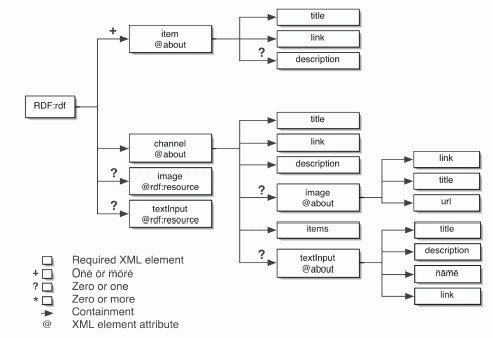
\includegraphics[scale=0.8]{rss091}
	}
	\captionof{figure}{Elementos que componen un canal de noticias RSS 0.91}
	\source{fuente: \cite{johnson2006rss}}
	\label{Elementos que componen un canal de noticias RSS 0.91}
\end{minipage}


\section{RSS 1.0}

Otros desarrolladores importantes, entre ellos Rael Dornfest, que 
trabajaba como director de tecnolog\'{i}a de O'Reilly, quer\'{i}a ampliar el 
alcance de RSS utilizando para otro prop\'{o}sito y lo conectan con formatos
adicionales. Por lo tanto, se dio introducci\'{o}n RDF \footnote{RDF :Resource
Description Framework Schema un set de clases con ciertas propiedades.} y 
tambi\'{e}n introdujo un nuevo mecanismo, el espacio de nombres XML. Una 
especificaci\'{o}n relacionado fue publicado en diciembre de 2002; los 
desarrolladores llaman el formato que se describe, RSS 1.0.\cite{johnson2006rss}

Esta norma, lanzado en diciembre de 2000, trajo dos cambios importantes en el 
mundo RSS: la introducci\'{o}n de RDF y con ella una introducci\'{o}n de espacios
de nombres.\cite{hammersley2005developing}
 
\subsection{Los elementos de RSS 1.0}

Comparando los RSS 0.91 y RSS 1.0 diagramas, tu puedes ver los formatos son significativos
diferentes. Son las diferencias:

\begin{itemize}

\item Un típico flujo RS 1.0 es más largo y más complejo, pero no lo hace incluir
tantos metadatos como el equivalente RSS 0.91 newfeed.

\item RSS 1.0 es más complejo, pero sólo porque es más flexible y extensible.

\item El elemento raíz es <RDF:rdf>  en lugar de <rss>.

\item Las noticias existen como hijos de elemento raíz del documento y no como 
hijos del elemento <channel>,como lo hacen en RSS 0.91.

\item Las noticias deben ser declaradas dentro del <channel> como recursos DRF. \par

En la Figura \ref{Los elementos XML que componen RSS 1.0}, para la composici\'{o}n
de un feed se tiene como primera categor\'{i}a la informaci\'{o}n sobre el canal 
de noticias y como segunda categor\'{i}a la informaci\'{o}n sobre los elementos.
En la primera  categor\'{i}a se observa un documento RDF seguido de <channel> la
cual se compone de: <title>, <link> y <description>. Como segunda categor\'{i}a 
se tiene a <item> que se tiene especificado con un rdf:about el cual compone de:
<title> , <link> lleva un permamente enlace y <description>. 

\begin{minipage}{1.0\linewidth}
	\centering
	\fbox{
		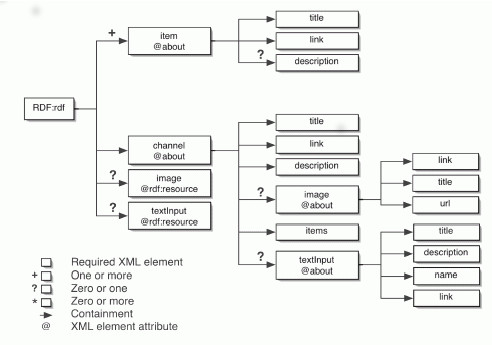
\includegraphics[scale=0.8]{rss010}
	}
	\captionof{figure}{Los elementos XML que componen RSS 1.0}
	\source{fuente: \cite{johnson2006rss}}
	\label{Los elementos XML que componen RSS 1.0}
\end{minipage}

\item <image> y <textInput> elementos deberian ser declarado dentro los <RDF:rdf>
elementos son RDF si han de ser incluidos dentro del <channel> elemento.

\item Muchos elementos de metadatos, tales como  <pubDate>, <lastBuild-Time>, 
<skipDays>, <skipHours>, <managingEditor>, y <webMaster> faltan de formato.
Estos se pueden a\~{n}adir seg\'{u}n sea necesario mediante el uso de RSS 1.0.
\cite{johnson2006rss}

\end{itemize}

\section{RSS 2.0}

Se tiene RSS 2.0 esencialmente define sintaxis, El soporte de RSS 2.0 es considerado
de baja especificaci\'{o}n ya que es uno de los formatos de mayores ventajas.

Hoy en d\'{i}a, es el formato RSS feed m\'{a}s utilizado. Es caracter\'{i}stico de
este formato no especifique, o para dejar a los desarrolladores de aplicaciones para
especificar: las conexiones entre Datos RSS, por una parte, entre otros formatos de
contenido, datos/formatos de metadatos, y entornos de publicaci\'{o}n.\cite{wittenbrink2005rss}

\subsection{Los elementos de RSS 2.0}

\'{U}ltimamente RSS es ampliamente usado. Las conexiones entre RSS datos, contenidos
de datos en formatos/metadatos en otros entornos.

Hoy en d\'{i}a, es el formato RSS m\'{a}s utilizado. Es caracter\'{i}stico de este
formato no especifique, o para dejar a los desarrolladores de aplicaciones para 
especificar: las conexiones entre Datos RSS, por una parte, entre otros formatos
de contenido, datos/formatos de metadatos, y entornos de publicaci\'{o}n, por otro
lado. Esencialmente, RSS 2.0 define la sintaxis, en tanto que significado y el uso
de determinaron mediante el uso de ejemplos. Los partidiarios de RSS 2.0 consideran
este bajo nivel de especificaci\'{o}n de una de las mayores ventajas del formato, 
mientras que los partidiarios de las versiones de RSS alternas ven como su mejor
momento en debilidad.\cite{wittenbrink2005rss}

Esto, en realidad es la clave para el \'{e}xito de la RSS 2.0. La cosa m\'{a}s simple
hay que hacer para hacer la validaci\'{o}n de alimentaci\'{o}n es muy sencillo de 
hecho. Si bien esto no es ninguna ayuda cuando usted est\'{a}
tratando de transmitir informaci\'{o}n compleja, como con RSS 1.0 o si usted est\'{a}
tratando de construir un sistema centrada en el documento completo, al igual que con
Atom, es muy \'{u}til para muchas otras aplicaciones.\cite{hammersley2005developing}

Los RSS 2.0 especificación provee una detallada descripci\'{o}n de cada elemento 
permitido en un RSS 2.0 newfeed. Tu puedes encontrar la especificaci\'{o}n aqu\'{i} 
RSS2.0 \footnote{RSS2.0:http://blogs.law.harvard.edu/tech/rss}. Figura \ref{Los 
elementos XML que componen RSS 2.0} resumiendo el XML que componen RSS 2.0, 
usando la misma notaci\'{o}n como nuestra previa figura.\cite{johnson2006rss}

Se tiene un nueva versi\'{o}n la cual conlleva las ventajas de las anteriores versiones
y esta pueda ser manipulable por lectores en equipos como agregadores online, tambi\'{e}n
implementadas en applicaciones web.

En la Figura \ref{Los elementos XML que componen RSS 2.0}, Se tiene el primera categor\'{i}a
se tiene informaci\'{o}n respecto al canal de noticias y como segunda categor\'{i}a los 
elementos de noticias que lo componen. Se habla sobre un canal de noticias conformado por
lo siguientes componentes: <title>, <link> y <description> requeridos. Se tiene como elemento
la etiqueta <item> comformado por los componenetes <title> y <description> minimamente un ejemplar.

\begin{minipage}{1.0\linewidth}
	\centering
	\fbox{
		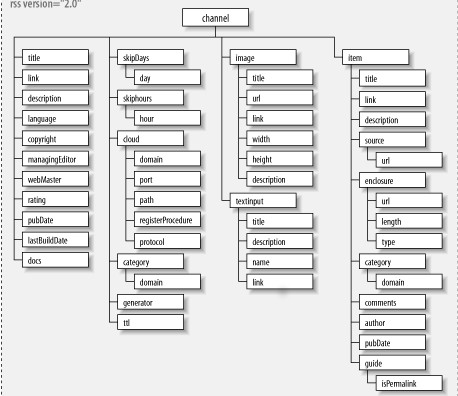
\includegraphics[scale=1.0]{rss020}
	}
	\captionof{figure}{Los elementos XML que componen RSS 2.0}
	\source{fuente: \cite{johnson2006rss}}
	\label{Los elementos XML que componen RSS 2.0}
\end{minipage}

\subsection{Plataforma Educativa LAEL}

En la Figura \ref{Subscripci\'{o}n Programa Aprendizaje Frances B\'{a}sico}. Se
tiene la realizaci\'{o}n de la subscripci\'{o}n de un canal de noticias, para 
ello el usuario deber\'{i}a ser autentificado. 

\begin{minipage}{1.0\linewidth}
	\centering
	\fbox{
		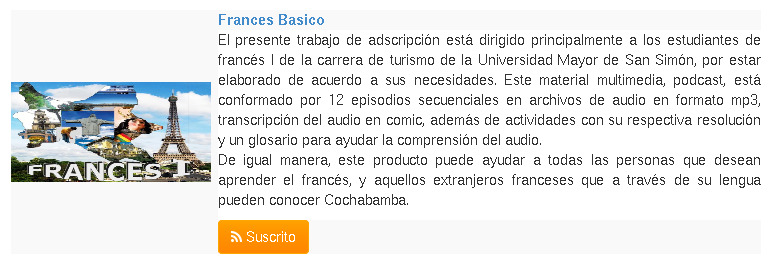
\includegraphics[scale=0.5]{basicFranceSubscribed}
	}
	\captionof{figure}{Subscripci\'{o}n Programa Aprendizaje Frances B\'{a}sico}
	\source{fuente: (Elaboraci\'{o}n Propia)}
	\label{Subscripci\'{o}n Programa Aprendizaje Frances B\'{a}sico}
\end{minipage}

En la Figura \ref{Episodio1: Elemento canal de noticias}. Se tiene uso de un navegador
como Firefox, se puede utilizar un lector de noticias que encuentra disponible y poder
identifcar los diferentes elementos que contiene un feed de noticas: T\'{i}tulo, Fecha
Liberaci\'{o}n y Descripci\'{o}n.
 
\begin{minipage}{1.0\linewidth}
	\centering
	\fbox{
		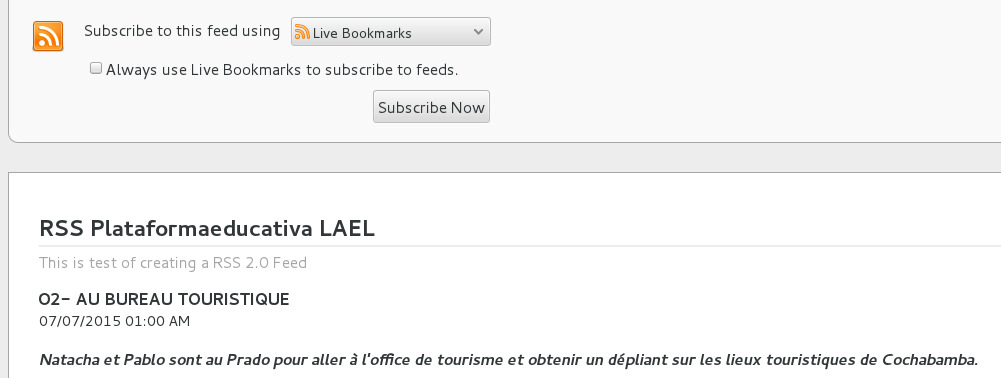
\includegraphics[scale=0.4]{basicFranceRssFirefox}
	}
	\captionof{figure}{Episodio1: Elemento canal de noticias}
	\source{fuente: (Elaboraci\'{o}n Propia)}
	\label{Episodio1: Elemento canal de noticias}
\end{minipage}


\subsection{Las nueve versiones incompatibles de RSS}

Un influente blogger Mark Pilgrim tiene que ser seguidor sobre desarrollado de RSS,
y el tiene que hacer algunas importantes contribuciones. Trabajando con Sam Ruby,
otro influente blogger, Pilgrim desarrollo servicio validaci\'{o}n de noticias versiones
\footnote{versiones: http://www.feedvalidator.org/} que maneja com\'{u}nmente uso de RSS
y Atom formato noticia. Pilgrim se\~{n}alo que hab\'{i}a nueve incompatibilidades en
versiones de RSS. Resumiendo estas incompatibles versiones y autores, fecha y estado
de cada una.\cite{johnson2006rss}

\begin{minipage}[b]{\hsize}\centering

\begin{tabular}{>{\centering\arraybackslash}m{.05\linewidth} |>{\centering\arraybackslash}m{.17\linewidth}|>{\centering\arraybackslash}m{.1\linewidth}|>{\centering\arraybackslash}m{.2\linewidth}|>{\centering\arraybackslash}m{.4\linewidth}}

& \textbf{Liberado por} & \textbf{Fecha} & \textbf{Estado} & \textbf{Nota} \\
\hline

\textbf{RSS 0.90} & Libby/Netscape & Enero 1999 & \textbf{Obsoleto} y rara vez se encuentra en la naturaleza & RDF- basado formato. \\
\hline

\textbf{RSS 0.91 } & Libby/Netscape & Julio 1999 & \textbf{Obsoleto} pero ampliamente usado & XML-basado con DTD; caído todos los elementos RDF; Añadido soporte para módulos. \\
\hline 

\textbf{RSS 0.91 (UserLand) } & Winer/Userland & Junio 2000 & \textbf{Obsoleto} pero ampliamente usado & caído DTD. \\
\hline 

\textbf{RSS 1.0} & RSS-DEV & Diciembre 2000 & \textbf{Viable} y ampliamente usado & RDF-basado formato nuevamente.\\
\hline

\textbf{RSS 0.92} & Winner/Userland & Diciembre 2000 & \textbf{Obsoleto} pero ampliamente usado & Contenido tipo de <description> elemento cambiado desde texto plano\\
\hline

\textbf{RSS 0.93} & Winer/Userland & Abril 2001 & \textbf{Obsoleto} y rara vez que se encuentra en la naturaleza & Aniadidp <pubDate> y <expirationDate> elementos. tambien permite multiples <enclousure> elementos por <item> \\
\hline

\textbf{RSS 0.94} & Winer/Userland & Verano 2002 & \textbf{Obsoleto} y rara vez que se encuentra en la naturaleza & eliminado <expirationDate> elemento. Especificación ya no está disponible en línea\\
\hline

\textbf{RSS 2.0} & Winer/Userland & Agosto 2002 & \textbf{Viable} y ampliamente usado. Final version de RSS & Permite adición de nuevos elementos siempre y cuando se definen por Espacio de nombres XML\\
\hline 

\textbf{RSS 2.0.1} & Winer/Harvard & Julio 2003 & Menor cambio a RSS 2.0 & Agregado elemento <rating>\\
\hline 

\end{tabular}

\captionof{table}{Las nueve versiones incompatibles de RSS}
\source{fuente: \cite{johnson2006rss}}
\end{minipage}

\section{El nuevo estandar: Atom}

A principios del 2003 un grupo de blooggers desilucionados con estado de newfeeds
publicaron un nuevo estandar API \footnote{API: Es un conjunto particular de reglas
y especificaci\'{o}n que el programas pueden seguir para comunicarse entre si} el
cual deberia ser conocido como Atom.

Atom es un formato de documento basado en XML que describe las listas de informaci\'{o}n
relacionada conocida como \textquotedblleft feeds\textquotedblright. Feeds se componen
de una serie de elementos, conocidos como \textquotedblleft entradas \textquotedblright,
cada uno con un conjunto extensible de metadatos adjunto.\cite{nottingham2005atom}

Si piensas Atom es una mejora sobre RSS o solamente otro formato, como un aplicación
de blog usted tendra que aprender Atom. Todo el mayor servidor blog si soporta Atom
ahora o tiene planes para hacer, y Blogger.com, uno de los largos servicios blogging,
ofrece solo Atom noticias - no RSS.\cite{johnson2006rss}

\subsection{Los elementos de Atom}

En la Figura \ref{Los elementos XML que conforman un servicio de noticias Atom}, 
se tiene como primera categor\'{i}a al <feed> como canal de noticas y sus datos
de informaci\'{o}n, como segunda categor\'{i}a se tiene los componentes un <entry>.
La primera categor\'{i}a comprende un <title>, <link>, <link> con la
propiedad rel="self", <update> y <autor>. En la segunda categor\'{i}a un elemento
<entry> esta compuesto por: <title>, <link>, <id>, <published> y <update> adem\'{a}s
de contener una subcategor\'{i}a denominada la etiqueta <content> con la propiedad
type="xhtml".

\begin{figure}[!ht]
	\centering
	\fbox{
		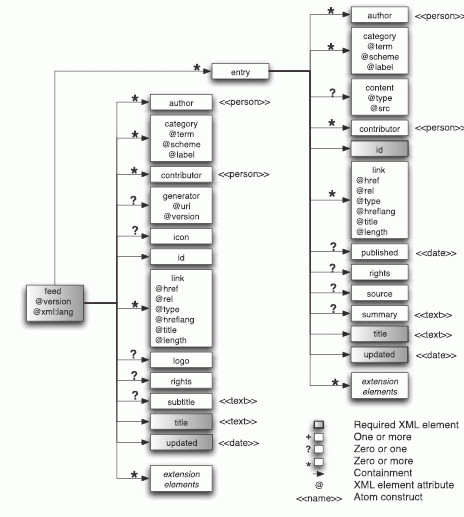
\includegraphics[scale=0.8]{elementsXML}
	}
	\caption{Los elementos XML que conforman un servicio de noticias Atom}
	\source{fuente: \cite{johnson2006rss}}
	\label{Los elementos XML que conforman un servicio de noticias Atom}
\end{figure}


Algunos requisitos importantes no son evidentes a partir de este diagrama formato
Atom, Por lo que se va revisar. En primer lugar, Primero, los requisitos de nivel feed.

\begin{itemize}

\item El feed debe contener un <id> elemento.
\item El feed debe contener un <link> con rel=\textquotedblleft self\textquotedblright 
que contiene un enlace del feed mismo. Esto hace posible para un programa, cual puede
tener solo una copia de un documento de noticias, a encontrar la URL de las noticias.
\item El feed debe incluir un solo enlace, significando un <link> elemento con rel=
\textquotedblleft alternate\textquotedblright - tipicamente un enlace alternativo de
un alimento hace referencia a una alternativa representación de la alimentación.
\item El autor debe ser especifico lugar el nivel feed o en cada individual entrada.

\end{itemize}

A continuaci\'{o}n se realiza un detalle de los elementos a considerar en cada nivel.

\begin{itemize}

\item Cada entrada debe contener un <id> elemento.
\item Si la entrada no tienen un <content> elemento, deberia tener una alternativo
enlace. Un enlace alternativo es su enalce permanente, un enlace permanente entradas
representacion web.
\item Un enlace puede tener multiples enlaces alternativos para diferentes lenguajes
y tipos de contenidos, pero una entrada deberia no contener mas que una enlace 
alternativo para cada combinacion de languages y tipo de contenido.
\item La entrada deberia incluir un <summary> elemento si el contenido es no 
facilmente leible, por ejemplo es no <content> elemento, el <content> elemento 
contiene algun otro texto, o el <content> referencia de elementos contenido en otros
lugares.\cite{johnson2006rss}

\end{itemize}

\subsection{Podcasting con Atom}


Podcasting originado como una caracteristica de RSS, pero a medida que el mundo se
mueve Atom como el nuevo estándar. Los podcasters también lo hará - y para buenas
razones. Atom puede soportar podcasting a travez del elemento <link>. Como es el
caso con RSS 2.0-basado podcasts, usted puedes tener solo un podcast por entrada.
Pero con Atom, tu puedes tener diferentes representacion por cada lenguage y por
cada tipo de contenido.\cite{johnson2006rss}

La Figura \ref{News feed árbol formato}, Se tiene la evoluci\'{o}n y los distintos
caminos tomados por los formatos por RSS y Atom en transcurir del tiempo

\begin{figure}[!htb]
	\centering
	\fbox{
		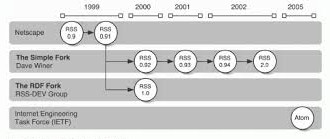
\includegraphics[scale=1]{newsFeed}
	}
	\caption{News feed árbol formato}
	\source{fuente: \cite{johnson2006rss}}
	\label{News feed árbol formato}
\end{figure}
